\section*{Zadanie 6}
Z ustalonego okręgu losujemy jednostajnie i niezależnie 3 punkty
\(A, B\) oraz \(C\). Jakie jest prawdopodobieństwo, że środek okręgu
leży wewnątrz trójkąta \(ABC\)?

\subsection*{Rozwiązanie}
Środek okręgu leży wewnątrz trójkąta, jeśli jest on ostrokątny. Nie może
mieć on łuku dłuższego niż połowa obwodu okręgu.

Bez straty ogólności niech punkt \(A\) będzie zawsze na lewo od środka okręgu
(\(A = (-r, 0)\)).

Bez straty ogólności niech \(B\) będzie na dolnym półokręgu.

Punkt \(C\) musi leżeć na krótszym łuku \(A'B'\) --- w przeciwnym
wypadku jeden z łuków \(AC\) lub \(BC\), niezawierający trzeciego
wierzchołka, byłby dłuższy niż połowa okręgu.

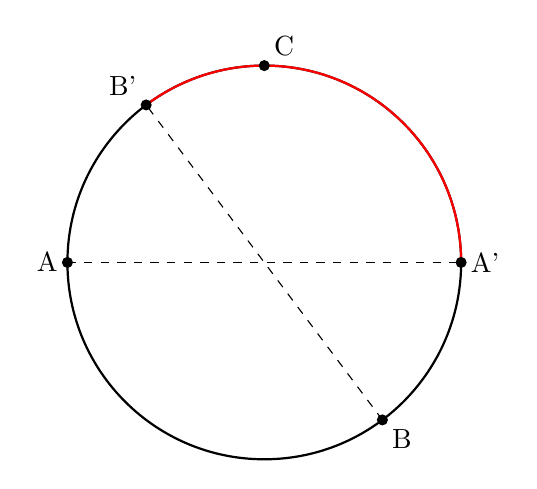
\begin{tikzpicture}
	\draw[thick] (0,0) circle(2.5cm);
	\draw[thick][red]
	(2.5,0) arc[start angle=0, end angle=127, radius=2.5cm];

	\fill (-2.5,0) circle (2pt) node[left] {A};
	\fill (1.5,-2) circle (2pt) node[below right] {B};
	\fill (0,2.5) circle (2pt) node[above right] {C};
	\fill (2.5,0) circle (2pt) node[right] {A'};
	\fill (-1.5,2) circle (2pt) node[above left] {B'};
	\draw[dashed] (-2.5,0) -- (2.5,0);
	\draw[dashed] (1.5,-2) -- (-1.5,2);

\end{tikzpicture}

Mając ustalony punkt \(A\) widzimy, że długość łuku \(AB\) jest
zmienną o rozkładzie jednostajnym na przedziale \([0, \pi r]\).

Dla dowolnego wyboru \(B\) prawdopodobieństwo, że \(C\) będzie dobre,
wynosi
\(\frac{\overset{\huge\frown}{A'B'}}{2\pi r}\)
\(= \frac{\overset{\huge\frown}{AB}}{2\pi r}\)

Średnia długość łuku to \(\frac{\pi r}2\), więc \(Pr = \frac 1 4\).

To widać, ale można ciut formalniej
\[
	\int_0^{\pi r} \frac{\frac{t}{\pi r}}{2\pi r}~dt
	= \frac{1}{2\pi^2r^2} \int_0^{\pi r} t~dt
	= \frac{1}{2\pi^2r^2} \cdot \frac {\pi^2r^2}2
	= \frac{1}{4}
\]

Bardzo drobnymi zmianami można zmienić to rozumowanie na bardzo podobne
do rozwiązania zadania 7., co pozostawiam jako ćwiczenie dla czytelnika.

\subsection*{Odpowiedź}
\[
	\boxed{\frac 1 4}
\]
